% IEEE standard conference template; to be used with:
%   spconf.sty  - LaTeX style file, and
%   IEEEbib.bst - IEEE bibliography style file.
% --------------------------------------------------------------------------

\documentclass[letterpaper]{article}
\usepackage{spconf,amsmath,amssymb,graphicx}
\usepackage{graphicx}
\usepackage[export]{adjustbox}


% Example definitions.
% --------------------
% nice symbols for real and complex numbers
\newcommand{\R}[0]{\mathbb{R}}
\newcommand{\C}[0]{\mathbb{C}}

% bold paragraph titles
\newcommand{\mypar}[1]{{\bf #1.}}

% Title.
% ------
\title{Parallel SAT Solving}
%
% Single address.
% ---------------
\name{Jan Eberhardt, Jakub Lichman}
\address{Department of Computer Science\\ ETH Zurich\\Zurich, Switzerland}

% For example:
% ------------
%\address{School\\
%		 Department\\
%		 Address}
%
% Two addresses (uncomment and modify for two-address case).
% ----------------------------------------------------------
%\twoauthors
%  {A. Author-one, B. Author-two\sthanks{Thanks to XYZ agency for funding.}}
%		 {School A-B\\
%		 Department A-B\\
%		 Address A-B}
%  {C. Author-three, D. Author-four\sthanks{The fourth author performed the work
%		 while at ...}}
%		 {School C-D\\
%		 Department C-D\\
%		 Address C-D}
%

\begin{document}
%\ninept
%
\maketitle
%

The hard page limit is 6 pages in this style. Do not reduce font size
or use other tricks to squeeze. This pdf is formatted in the American letter format, so the spacing may look a bit strange when printed out.

\begin{abstract}
Describe in concise words what you do, why you do it (not necessarily
in this order), and the main result.  The abstract has to be
self-contained and readable for a person in the general area. You
should write the abstract last.
\end{abstract}

\section{Introduction}\label{sec:intro}

\mypar{Motivation} Boolean satisfiability problem (SAT) belongs to the most important problems in program analysis, verification and other disciplines of theoretical computer science. It is particularly used in background of many applications, especially ones in the field of automated planning and scheduling, model checking(formal verification) and theorem proving. 

Last decade brought many improvements to SAT world in form of advanced heuristics, preprocessing and inprocessing techniques and data structures that allow efficient implementation of search space pruning. 

However, past 10 years were also rich on improvements in parallelism. Current trends in computer hardware design decreased performance per processing unit and pack more units on a single processor. It is caused by thermal wall which stopped further increase of clock speed. However, algorithms for SAT solving like DPLL and CDCL were invented before wide use of parallelism and therefore were designed for sequential execution. Since SAT is a NP-complete problem, we consider it the right candidate for running in parallel.

In our approach, we are trying to speed up SAT solving by running it on multiple cores with different techniques of search space partitioning. Final comparison is done between different parallel versions and sequential one. Parallel versions are mainly based on DPLL algorithm except the one which uses also CDCL, but locally. All algorithms are unlimited in number of cores they can run on. However, some scale better than the others. 

Experiments were run on cluster where we were allowed to use at most 48 cores. Tests were taken from SATLIB - The Satisfiability Library \cite{cnf_website} and they were also created by our own random generator of formulas. Results show nice speedups in parallel versions against sequential one. However, parallel DPLL algorithm is still not able to outperform sequential CDCL. It shows how good CDCL actually is in comparison with DPLL. 

\mypar{Related work} Tomas Balyo et al. in their paper \cite{hordesat} propose HordeSat solver which can run up to 1024 cores and is based on CDCL algorithm. Their parallel approach is different from ours because it is portfolio based but with sign of search space partitioning. Most of the previous SAT solvers designed for computer clusters or grids use explicit search space partitioning. Examples of such solvers are GridSAT \cite{gridsat}, PMSAT \cite{pmsat} and many more. Paper that is probably closest to ours \cite{stealing} firstly introduced work stealing for dynamic load-balancing. 

\section{Background: Whatever the Background is}\label{sec:background}

//Jakubs version
SAT solver is program that is able to decide whether given formula is satisfiable i.e. there exists assignment of variables that makes whole formula true-satisfiable or not-unsatisfiable.
First algorithm was develop in 1960 by Martin Davis and Hilary Putnam for checking the validity of a first-order logic formula using a resolution-based decision procedure for propositional logic.
%[src: https://en.wikipedia.org/wiki/Davis%E2%80%93Putnam_algorithm].
Since Davis-Putnam algorithm was able to handle just valid formulas, more general procedure for SAT solving was needed. In 1962 was developed new, complete algorithm that was able to handle all types of formulas. The algorithm is called DPLL after Davis�Putnam�Logemann�Loveland. Its  backtracking-based search algorithm that still forms the basis for most efficient complete SAT solvers. Since DPLL invention there were many algorithms proposed, which improve runtime of SAT solving significantly.

\mypar{SAT}
The SAT problem is the following:
Given a propositional logic formula $F$ we try to find a valid assignment of variables $v_i$ of $F$.
A valid assignment is one that makes the formula $F$ true.
More formally: //TODO

The question that a SAT solver needs to answer is the following:
Given a formula $F$, is it satisfiable?
And if so what would be a valid variable assignment?

//TODO Nice small figure here

\mypar{DPLL}
The Davis Putnam Logemann Loveland algorithm, or short DPLL, was introduced by M. Davis, G. Logemann and D. Loveland in 1962. \cite{dpll}
It is an extension of the Davis and Putnam, or short DP, algorithm. \cite{dp}
DPLL solves a SAT problem by modelling it as a decision tree, variables can either be assigned \texttt{true} or \texttt{false}.
In every step DPLL tries to find variables that are "automatically" assigned because of a previous decision,
if there are none it will pick a variable $v_i$ and assume a value for it.
If it later turns out that this decision was wrong it backtracks to that point and picks the negated assignment for variable $v_i$.
\mypar{CDCL}
//TODO \cite{cdcl}

\section{Parallelizing DPLL}\label{sec:parallel_dpll}

We decided to parallelize DPLL because it is a relatively simple backtracking algorithm and therefore it does not require any advanced communication.
Subtasks can be solved individually and therefore also on different nodes.

\mypar{DPLL Branches}
As introduced in Section \ref{sec:background} the DPLL algorithm at some point needs to make a decision.
If there are no more variables that can be assigned trivially, we need to pick one variable and just assume that it is either \texttt{true} or \texttt{false}.
That is exactly the point where we can let some other node solve the other branch.
We looked at two different ways on how to split the work between multiple nodes.
Firstly a master slave communication pattern, where one node is in charge of storing partial models and eventually passing them on to a slave or worker that will solve it.
And secondly a work stealing scheduling communication model where each node runs on its own and if it runs out of work and the formula is not solved yet,
it picks a random other node and requests a partial model to work on from that node.

\mypar{Master Slave Model}
//TODO introduce the model and put a nice and compact figure here.

\mypar{Work Stealing Scheduler}
//TODO introduce the model and put a nice and compact figure here.
Our current work stealing implementation can only handle satisfiable cases.
The stopping criteria in the unsatisfiable case was very trivial in the master slave model, however in the work stealing scheduler it is not trivial:
How does one detect if all workers are asking other workers for work, but no worker has work left?
Currently we just ignore this case.

\mypar{Implementation}
We implemented both communication models in C++ with MPI \cite{mpi}.
Our DPLL solver is also implemented in C++ and therefore we can directly interact with MPI from within the solver.
Our DPLL implementation is straight forward and simple, we use \texttt{vector}s from the C++ standard library to represent sets of clauses and sets of literals.
We use \texttt{unsigned int}s as variable names, and boolean values for sign and value of the literal and variable.
To implement the backtracking algorithm we use recursion, but allocate all necessary data structures on the heap.
We didn't experience any stack overflow issues.

\mypar{Correctness}
We tested our sequential DPLL solver on hundreds of formulas that we either randomly generated ourselves or took over from a DIMACS formula collection. \cite{cnf_website}
We ran each formula through z3 \cite{z3} and compared the result of z3 with our result.
The following cases have to be considered for each test case:
\begin{itemize}
    \item If both solvers return unsat, we pass the test case.
    \item If one solver returns sat and the other one unsat, we fail the test case.
    \item If both solvers return sat, we still need to check if the model our solver has returned is correct.
        To do that we can conjoin the model to the original formula and again run it through z3.
\end{itemize}

We ran the both parallel implementations through the same set of formulas and checked also for each of them that they are correctly solved.
Assuming that our sequential implementation is correct, it is straight forward that our parallel implementation is also correct, since we essentially just solve subproblems with the sequential version.
All steps of the algorithm stay unchanged, we just store the "other" branch (reformulate this) in a different data structure and resume it potentially at a different point in time.


\section{Experimental Results}\label{sec:exp}

We ran both communication models on the Euler super compute cluster. \cite{euler}.

\mypar{Experimental Setup}
We ran our implementation on up to 48 cores, which was the maximum accessible to us on Euler, and requested 1 Gigabyte of memory per core.
//TODO talk about processors, clock frequencies, OS etc necessary?

During our correctness testing and debugging phase of the core algorithm, we realized that random formulas are not a particular good fit to test performance.
At least not the kind of random formulas that we generated with our own random formula generator.
Even though they used the same amount of variables, clauses and literals per clause the runtimes varied quite a bit because the problems had a completely randoms structure.
We used a set of XX formulas in the DIMACS CNF format as a benchmark set.
The set contains different real world problems from various domains such as //TODO.

\mypar{Master Slave}
We compared the runtimes of the master slave communication pattern with sequential DPLL.
//Question to answer: How well do we scale?
The speedup that we achieve is shown in Figure \ref{fig:dpll_parallel_speedup} on a representable subset of the benchmark set.
\begin{figure}
    \centering
    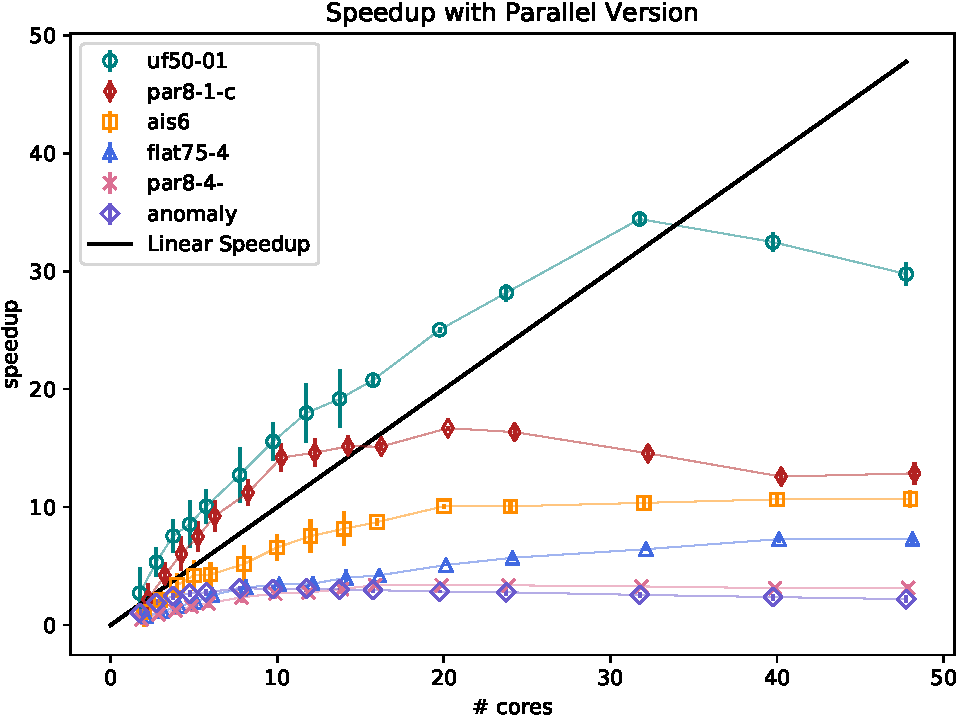
\includegraphics[width=\columnwidth]{figures/dpll_scaling_parallel}
    \caption{Speedup of master slave parallel DPLL implementation compared to sequential DPLL.
    \label{fig:dpll_parallel_speedup}}
\end{figure}
The speedup factor that we achieved heavily depends on the formula.
But it is not just the "size" of the problem or time required to solve a formula that influences the speedup factor.
As shown in Table \ref{tab:cnfs_parallel} the formulas where we reached the highest speedup are not necessarily the ones with the largest number of variables or longest time to solve sequentially.
Note that the best speedup in this subset is actually achieved for the formula that is randomly generated.

\begin{table}
    \centering
    \begin{tabular}{|l|c|c|c|}
        \hline
        formula & avg. runtime & \# vars/clauses & \# decisions \\
        \hline
        \hline
        uf50-01 & todo & 50/218 & 286\\
        \hline
        par8-1-c & todo & 64/254 & 32 \\
        \hline
        ais6 & todo & 61/581 & 30 \\
        \hline
        flat75-4 & todo & 225/840 & 31\\
        \hline
        par8-4- & todo & 67/266 & 19 \\
        \hline
        anomaly & todo & 48/261 & 5 \\
        \hline
    \end{tabular}
    \caption{Overview of benchmark subset formulas.}
    \label{tab:cnfs_parallel}
\end{table}

//TODO

//Question to answer: when does master become a bottleneck
\begin{figure}
    \centering
    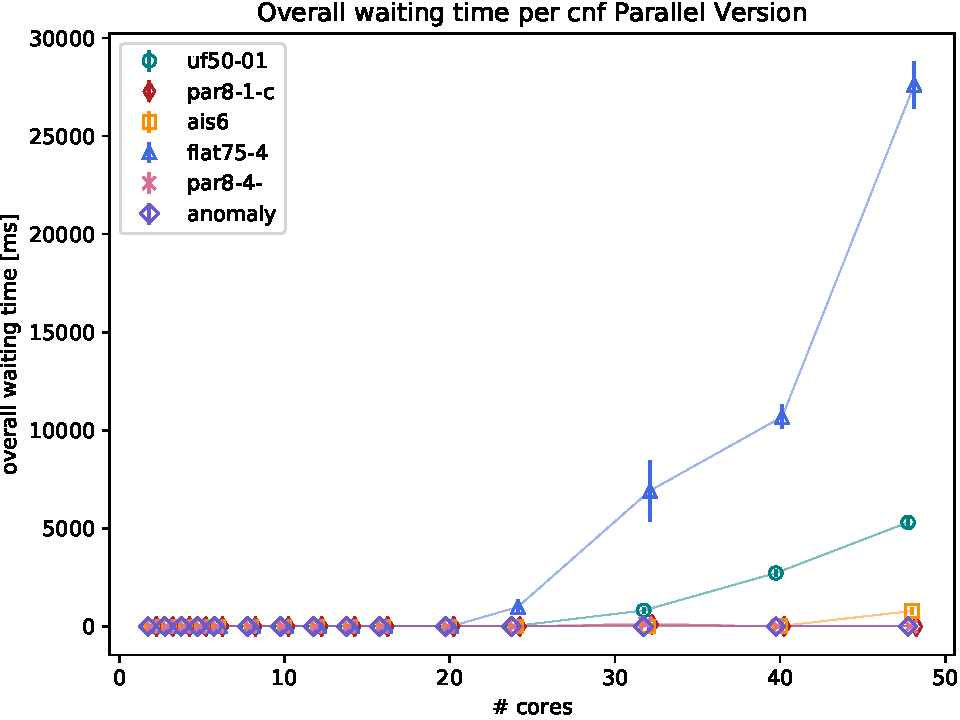
\includegraphics[width=\columnwidth]{figures/dpll_waiting_parallel}
    \caption{Overall waiting time of workers per cnf in parallel Version.
    All waiting times per worker are summed up.
    \label{fig:dpll_parallel_waiting}}
\end{figure}

\mypar{Stealing Scheduling}
Similar to the previous comparison, we compared the parallel work stealing algorithm to sequential DPLL.
\begin{figure}
  \centering
  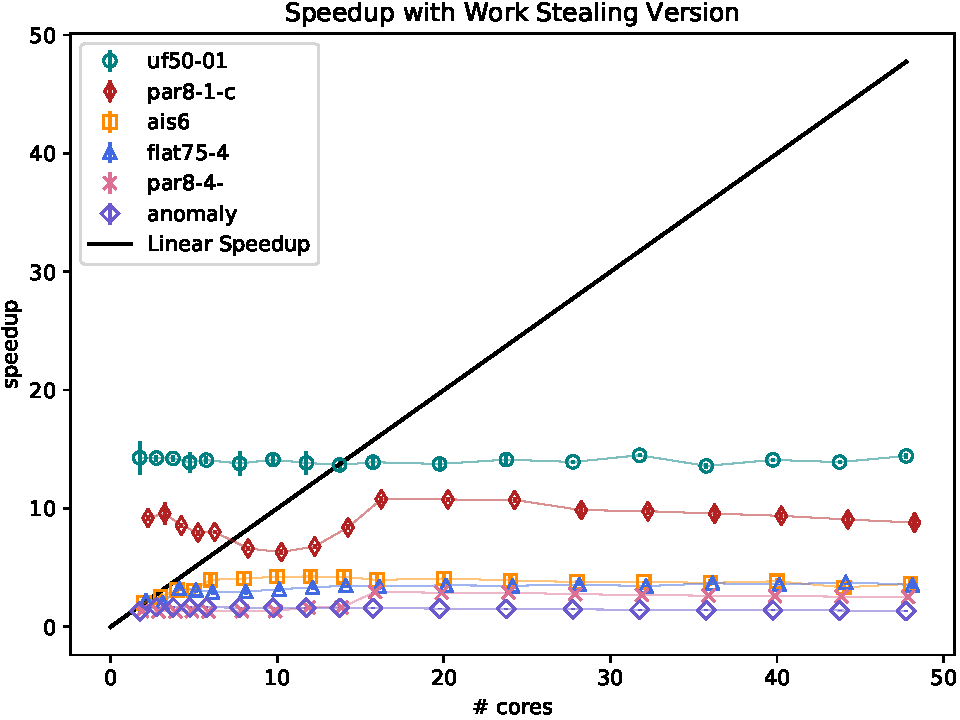
\includegraphics[width=\columnwidth]{figures/dpll_scaling_stealing}
  \caption{Speedup of work stealing parallel DPLL implementation compared to sequential DPLL.
  \label{fig:dpll_stealing_speedup}}
\end{figure}
//Question to answer: How well do we scale?

\section{Conclusions}

Here you need to summarize what you did and why this is
important. {\em Do not take the abstract} and put it in the past
tense. Remember, now the reader has (hopefully) read the report, so it
is a very different situation from the abstract. Try to highlight
important results and say the things you really want to get across
such as high-level statements (e.g., we believe that .... is the right
approach to .... Even though we only considered x, the
.... technique should be applicable ....) You can also formulate next
steps if you want. Be brief. After the conclusions there are only the references.

\section{Further comments}

Here we provide some further tips.

\mypar{Further general guidelines}

\begin{itemize}
\item For short papers, to save space, I use paragraph titles instead of
subsections, as shown in the introduction.

\item It is generally a good idea to break sections into such smaller
units for readability and since it helps you to (visually) structure the story.

\item The above section titles should be adapted to more precisely
reflect what you do.

\item Each section should be started with a very
short summary of what the reader can expect in this section. Nothing
more awkward as when the story starts and one does not know what the
direction is or the goal.

\item Make sure you define every acronym you use, no matter how
convinced you are the reader knows it.

\item Always spell-check before you submit (to us in this case).

\item Be picky. When writing a paper you should always strive for very
high quality. Many people may read it and the quality makes a big difference.
In this class, the quality is part of the grade.

\item Books helping you to write better: \cite{Higham:98} and \cite{Strunk:00}.

\item Conversion to pdf (latex users only): 

dvips -o conference.ps -t letter -Ppdf -G0 conference.dvi

and then

ps2pdf conference.ps
\end{itemize}

\mypar{Graphics} For plots that are not images {\em never} generate the bitmap formats
jpeg, gif, bmp, tif. Use eps, which means encapsulate postscript. It is
scalable since it is a vector graphic description of your graph. E.g.,
from Matlab, you can export to eps.

The format pdf is also fine for plots (you need pdflatex then), but only if the plot was never before in the format 
jpeg, gif, bmp, tif.


% References should be produced using the bibtex program from suitable
% BiBTeX files (here: bibl_conf). The IEEEbib.bst bibliography
% style file from IEEE produces unsorted bibliography list.
% -------------------------------------------------------------------------
\bibliographystyle{IEEEbib}
\bibliography{bibl_conf}

\end{document}

